\subsection{Load step}
Igen er load steppet realiseret som det blev gjort i load step sektionen ~\ref{loadsteprea} under 2. iteration. Resultatet af dette ses på figur~\ref{fig:Loadstep3}
\begin{figure}[H]
	\center
	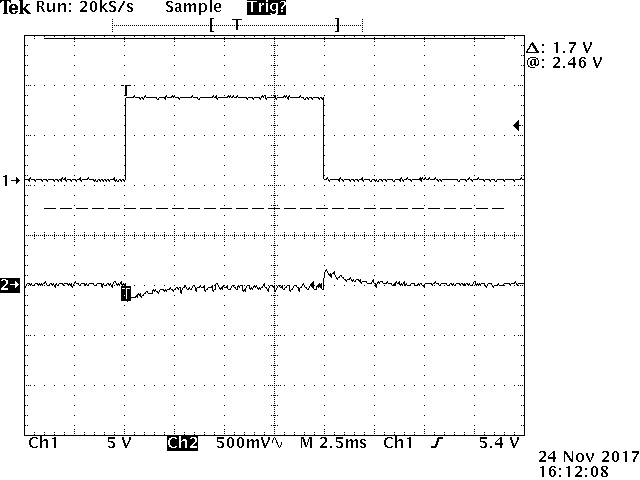
\includegraphics[max width=0.7\linewidth]{/tex/3iteration/billeder/realisering/Loadstep.PNG}
	\caption{Realiseret load step}
	\label{fig:Loadstep3}
\end{figure} 
\noindent Det er tydeligt at overshootet er faldet en del med den større båndbredde. På ~\ref{fig:Loadsteprise} er der zoomet ind på dykket, som er der hvor loaden skifter til $10\ohm$.
\begin{figure}[H]
	\center
	\includegraphics[max width=0.7\linewidth]{/tex/3iteration/billeder/realisering/Loadsteprise.PNG}
	\caption{Zoom på dyk ved $10\ohm$}
	\label{fig:Loadsteprise}
\end{figure}

\noindent Dette dyk aflæses til at være ca. $300mV$, hvilket skal ses i forhold til de $700mV$ fra tidligere. Til gengæld er reguleringstiden steget med omkring $0.5ms$ til $2ms$. På ~\ref{fig:Loadstepfall} ses i stedet stigningen, da loaden igen hæve til $20\ohm$.
\begin{figure}[H]
	\center
	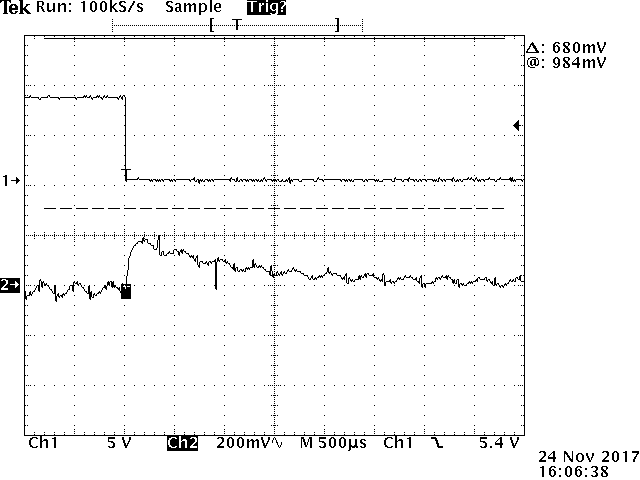
\includegraphics[max width=0.7\linewidth]{/tex/3iteration/billeder/realisering/Loadstepfall.PNG}
	\caption{Zoom på stigning ved $20\ohm$}
	\label{fig:Loadstepfall}
\end{figure}

\noindent Her aflæses stigningen til $200mV$ i forhold til de tidligere $600mV$ og igen er reguleringstiden steget med ca. $0.5ms$ til $2ms$. 